
\newcommand{\figureHAAlphaDiagram}
{
\tikzset{every picture/.style={line width=0.75pt}} %set default line width to 0.75pt        

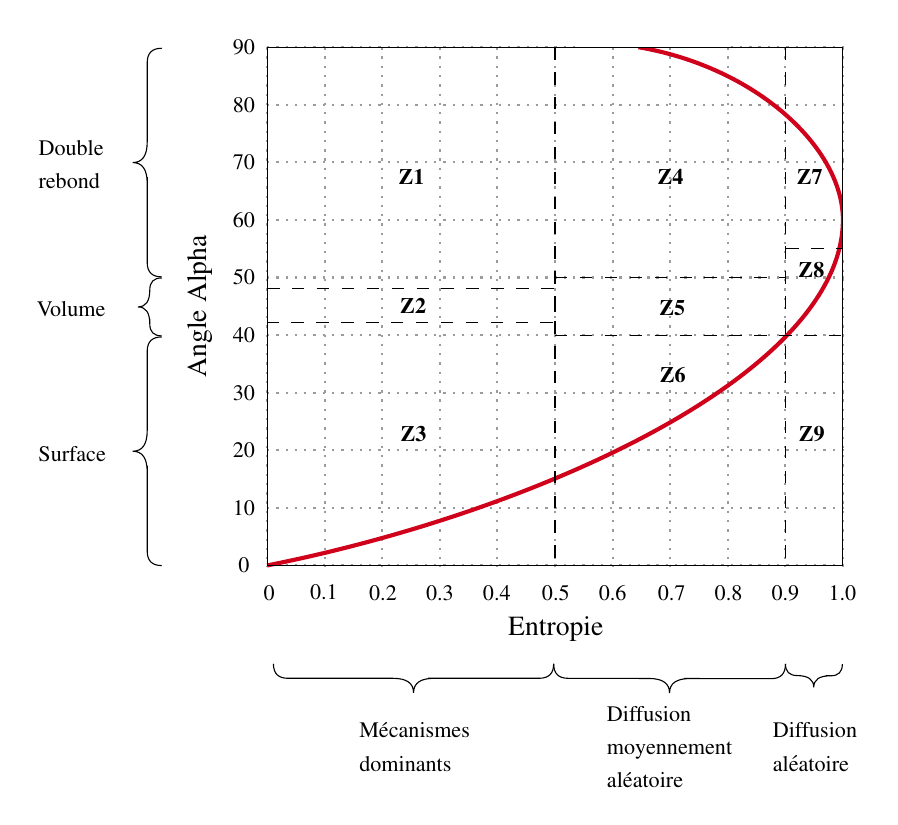
\begin{tikzpicture}[x=0.75pt,y=0.75pt,yscale=-1,xscale=1]
%uncomment if require: \path (0,403); %set diagram left start at 0, and has height of 403

%Shape: Grid [id:dp5329817915715289] 
\draw  [draw opacity=0][dash pattern={on 0.84pt off 2.51pt}][line width=0.75]  (132.39,30.81) -- (411.21,30.81) -- (411.21,280.96) -- (132.39,280.96) -- cycle ; \draw  [color={rgb, 255:red, 155; green, 155; blue, 155 }  ,draw opacity=1 ][dash pattern={on 0.84pt off 2.51pt}][line width=0.75]  (132.39,30.81) -- (132.39,280.96)(160.14,30.81) -- (160.14,280.96)(187.88,30.81) -- (187.88,280.96)(215.62,30.81) -- (215.62,280.96)(243.37,30.81) -- (243.37,280.96)(271.11,30.81) -- (271.11,280.96)(298.85,30.81) -- (298.85,280.96)(326.6,30.81) -- (326.6,280.96)(354.34,30.81) -- (354.34,280.96)(382.08,30.81) -- (382.08,280.96)(409.83,30.81) -- (409.83,280.96) ; \draw  [color={rgb, 255:red, 155; green, 155; blue, 155 }  ,draw opacity=1 ][dash pattern={on 0.84pt off 2.51pt}][line width=0.75]  (132.39,30.81) -- (411.21,30.81)(132.39,58.55) -- (411.21,58.55)(132.39,86.3) -- (411.21,86.3)(132.39,114.04) -- (411.21,114.04)(132.39,141.78) -- (411.21,141.78)(132.39,169.53) -- (411.21,169.53)(132.39,197.27) -- (411.21,197.27)(132.39,225.01) -- (411.21,225.01)(132.39,252.76) -- (411.21,252.76)(132.39,280.5) -- (411.21,280.5) ; \draw  [color={rgb, 255:red, 155; green, 155; blue, 155 }  ,draw opacity=1 ][dash pattern={on 0.84pt off 2.51pt}][line width=0.75]   ;
%Curve Lines [id:da4332063526878951] 
\draw [color={rgb, 255:red, 208; green, 2; blue, 27 }  ,draw opacity=1 ][line width=1.5]    (311.34,30.81) .. controls (368.21,40.52) and (409.83,79.36) .. (409.83,114.04) ;


%Curve Lines [id:da34601885617547357] 
\draw [color={rgb, 255:red, 208; green, 2; blue, 27 }  ,draw opacity=1 ][line width=1.5]    (132.39,280.5) .. controls (258.62,255.53) and (409.38,189.52) .. (409.83,114.04) ;


%Straight Lines [id:da5416227795128452] 
\draw  [dash pattern={on 4.5pt off 4.5pt}]  (271.11,30.81) -- (271.11,280.5) ;


%Straight Lines [id:da030952056784959048] 
\draw  [dash pattern={on 4.5pt off 4.5pt}]  (382.08,30.81) -- (382.08,280.5) ;


%Straight Lines [id:da7286341961263789] 
\draw  [dash pattern={on 4.5pt off 4.5pt}]  (271.11,141.78) -- (382.08,141.78) ;


%Straight Lines [id:da39527812824722464] 
\draw  [dash pattern={on 4.5pt off 4.5pt}]  (271.11,169.53) -- (409.83,169.53) ;


%Straight Lines [id:da6097088102452988] 
\draw  [dash pattern={on 4.5pt off 4.5pt}]  (382.47,127.75) -- (409.88,127.75) ;


%Shape: Rectangle [id:dp09011117578889105] 
\draw  [dash pattern={on 4.5pt off 4.5pt}] (132.39,147.16) -- (271.11,147.16) -- (271.11,163.44) -- (132.39,163.44) -- cycle ;
%Shape: Brace [id:dp38044155871255403] 
\draw   (81.63,31.32) .. controls (76.96,31.32) and (74.63,33.65) .. (74.63,38.32) -- (74.63,76.39) .. controls (74.63,83.06) and (72.3,86.39) .. (67.63,86.39) .. controls (72.3,86.39) and (74.63,89.72) .. (74.63,96.39)(74.63,93.39) -- (74.63,134.47) .. controls (74.63,139.14) and (76.96,141.47) .. (81.63,141.47) ;
%Shape: Brace [id:dp619029032090431] 
\draw   (81.63,170.4) .. controls (76.96,170.4) and (74.63,172.73) .. (74.63,177.4) -- (74.63,215.48) .. controls (74.63,222.15) and (72.3,225.48) .. (67.63,225.48) .. controls (72.3,225.48) and (74.63,228.81) .. (74.63,235.48)(74.63,232.48) -- (74.63,273.56) .. controls (74.63,278.23) and (76.96,280.56) .. (81.63,280.56) ;
%Shape: Brace [id:dp663391190432135] 
\draw   (81.63,141.98) .. controls (77.8,141.98) and (75.88,143.9) .. (75.88,147.73) -- (75.88,147.73) .. controls (75.88,153.2) and (73.96,155.94) .. (70.13,155.94) .. controls (73.96,155.94) and (75.88,158.68) .. (75.88,164.15)(75.88,161.68) -- (75.88,164.15) .. controls (75.88,167.98) and (77.8,169.9) .. (81.63,169.9) ;
%Shape: Brace [id:dp4085062930632537] 
\draw   (135.44,327.87) .. controls (135.44,332.54) and (137.77,334.87) .. (142.44,334.87) -- (192.95,334.87) .. controls (199.62,334.87) and (202.95,337.2) .. (202.95,341.87) .. controls (202.95,337.2) and (206.28,334.87) .. (212.95,334.87)(209.95,334.87) -- (263.46,334.87) .. controls (268.13,334.87) and (270.46,332.54) .. (270.46,327.87) ;
%Shape: Brace [id:dp24103434780275457] 
\draw   (270.46,327.87) .. controls (270.45,332.54) and (272.78,334.87) .. (277.45,334.88) -- (316.29,334.95) .. controls (322.96,334.96) and (326.29,337.29) .. (326.28,341.96) .. controls (326.29,337.29) and (329.62,334.97) .. (336.29,334.98)(333.29,334.98) -- (375.13,335.05) .. controls (379.8,335.06) and (382.13,332.73) .. (382.14,328.06) ;
%Shape: Brace [id:dp11940710267920851] 
\draw   (382.14,327.87) .. controls (382.11,331.63) and (383.98,333.52) .. (387.74,333.55) -- (387.74,333.55) .. controls (393.11,333.59) and (395.79,335.49) .. (395.76,339.25) .. controls (395.79,335.49) and (398.49,333.63) .. (403.86,333.67)(401.45,333.65) -- (403.86,333.67) .. controls (407.63,333.7) and (409.52,331.83) .. (409.55,328.07) ;
%Shape: Rectangle [id:dp9635876596122388] 
\draw  [draw opacity=0][fill={rgb, 255:red, 255; green, 255; blue, 255 }  ,fill opacity=1 ] (283.27,21.67) -- (354.34,21.67) -- (354.34,30.81) -- (283.27,30.81) -- cycle ;
%Shape: Rectangle [id:dp7125237452603193] 
\draw  [draw opacity=0][fill={rgb, 255:red, 255; green, 255; blue, 255 }  ,fill opacity=1 ] (409.88,92.74) -- (422.75,92.74) -- (422.75,133.35) -- (409.88,133.35) -- cycle ;
%Shape: Rectangle [id:dp191713542404937] 
\draw   (132.39,30.81) -- (409.83,30.81) -- (409.83,280.5) -- (132.39,280.5) -- cycle ;


% Text Node
\draw (121.22,30.81) node  [font=\footnotesize] [align=left] {{\fontfamily{ptm}\selectfont 90}};
% Text Node
\draw (121.22,58.55) node  [font=\footnotesize] [align=left] {{\fontfamily{ptm}\selectfont 80}};
% Text Node
\draw (121.22,86.3) node  [font=\footnotesize] [align=left] {{\fontfamily{ptm}\selectfont 70}};
% Text Node
\draw (121.22,114.04) node  [font=\footnotesize] [align=left] {{\fontfamily{ptm}\selectfont 60}};
% Text Node
\draw (121.22,141.78) node  [font=\footnotesize] [align=left] {{\fontfamily{ptm}\selectfont 50}};
% Text Node
\draw (121.22,169.53) node  [font=\footnotesize] [align=left] {{\fontfamily{ptm}\selectfont 40}};
% Text Node
\draw (121.22,197.27) node  [font=\footnotesize] [align=left] {{\fontfamily{ptm}\selectfont 30}};
% Text Node
\draw (121.22,252.76) node  [font=\footnotesize] [align=left] {{\fontfamily{ptm}\selectfont 10}};
% Text Node
\draw (121.22,225.01) node  [font=\footnotesize] [align=left] {{\fontfamily{ptm}\selectfont 20}};
% Text Node
\draw (121.22,280.5) node  [font=\footnotesize] [align=left] {{\fontfamily{ptm}\selectfont 0}};
% Text Node
\draw (159.8,293.37) node  [font=\footnotesize] [align=left] {{\fontfamily{ptm}\selectfont 0.1}};
% Text Node
\draw (188.23,293.75) node  [font=\footnotesize] [align=left] {{\fontfamily{ptm}\selectfont 0.2}};
% Text Node
\draw (215.64,293.75) node  [font=\footnotesize] [align=left] {{\fontfamily{ptm}\selectfont 0.3}};
% Text Node
\draw (243.05,293.75) node  [font=\footnotesize] [align=left] {{\fontfamily{ptm}\selectfont 0.4}};
% Text Node
\draw (271.48,293.75) node  [font=\footnotesize] [align=left] {{\fontfamily{ptm}\selectfont 0.5}};
% Text Node
\draw (298.89,293.75) node  [font=\footnotesize] [align=left] {{\fontfamily{ptm}\selectfont 0.6}};
% Text Node
\draw (327.32,293.75) node  [font=\footnotesize] [align=left] {{\fontfamily{ptm}\selectfont 0.7}};
% Text Node
\draw (354.73,293.75) node  [font=\footnotesize] [align=left] {{\fontfamily{ptm}\selectfont 0.8}};
% Text Node
\draw (382.14,293.75) node  [font=\footnotesize] [align=left] {{\fontfamily{ptm}\selectfont 0.9}};
% Text Node
\draw (409.55,293.75) node  [font=\footnotesize] [align=left] {{\fontfamily{ptm}\selectfont 1.0}};
% Text Node
\draw (133.41,293.7) node  [font=\footnotesize] [align=left] {{\fontfamily{ptm}\selectfont 0}};
% Text Node
\draw (99.9,155.65) node  [rotate=-270] [align=left] {{\fontfamily{ptm}\selectfont Angle Alpha}};
% Text Node
\draw (271.48,310.98) node   [align=left] {{\fontfamily{ptm}\selectfont Entropie}};
% Text Node
\draw (201.94,93.4) node  [font=\footnotesize] [align=left] {{\fontfamily{ptm}\selectfont \textbf{Z1}}};
% Text Node
\draw (202.77,155.3) node  [font=\footnotesize] [align=left] {{\fontfamily{ptm}\selectfont \textbf{Z2}}};
% Text Node
\draw (202.95,217.22) node  [font=\footnotesize] [align=left] {{\fontfamily{ptm}\selectfont \textbf{Z3}}};
% Text Node
\draw (326.81,93.4) node  [font=\footnotesize] [align=left] {{\fontfamily{ptm}\selectfont \textbf{Z4}}};
% Text Node
\draw (327.64,156.31) node  [font=\footnotesize] [align=left] {{\fontfamily{ptm}\selectfont \textbf{Z5}}};
% Text Node
\draw (327.82,188.8) node  [font=\footnotesize] [align=left] {{\fontfamily{ptm}\selectfont \textbf{Z6}}};
% Text Node
\draw (393.81,93.4) node  [font=\footnotesize] [align=left] {{\fontfamily{ptm}\selectfont \textbf{Z7}}};
% Text Node
\draw (394.64,138.04) node  [font=\footnotesize] [align=left] {{\fontfamily{ptm}\selectfont \textbf{Z8}}};
% Text Node
\draw (394.83,217.22) node  [font=\footnotesize] [align=left] {{\fontfamily{ptm}\selectfont \textbf{Z9}}};
% Text Node
\draw (37.98,87.29) node   [align=left] {{\fontfamily{ptm}\selectfont {\footnotesize Double}}\\{\fontfamily{ptm}\selectfont {\footnotesize rebond}}};
% Text Node
\draw (37.98,156.84) node   [align=left] {{\fontfamily{ptm}\selectfont {\footnotesize Volume}}};
% Text Node
\draw (38.48,226.89) node   [align=left] {{\fontfamily{ptm}\selectfont {\footnotesize Surface}}};
% Text Node
\draw (203.46,368) node   [align=left] {{\fontfamily{ptm}\selectfont {\footnotesize Mécanismes}}\\{\fontfamily{ptm}\selectfont {\footnotesize dominants}}};
% Text Node
\draw (326.3,368) node   [align=left] {{\footnotesize {\fontfamily{ptm}\selectfont Diffusion}}\\{\footnotesize {\fontfamily{ptm}\selectfont moyennement}}\\{\footnotesize {\fontfamily{ptm}\selectfont aléatoire}}};
% Text Node
\draw (396.35,368) node   [align=left] {{\footnotesize {\fontfamily{ptm}\selectfont Diffusion}}\\{\footnotesize {\fontfamily{ptm}\selectfont aléatoire}}};


\end{tikzpicture}

